\documentclass[12pt]{article}
\usepackage[paper=letterpaper, left=1in, right=1in, top=1in, bottom=1in]{geometry}

\usepackage[parfill]{parskip}
\usepackage{amsmath}
\usepackage{graphicx}

\begin{document}
\thispagestyle{empty}

\begin{center}
{\large CS 310}\\
Assignment 210
\end{center}

\begin{flushright}
Hieu Le
\end{flushright}

Program 210 implements an algorithm to determine the largest integral
power of 2 smaller than or equal to an arbitrary non-negative
integer $n$. It does so by iteratively clearing the least significant set bit 
in the binary representation of the variable $j$, which is initially set to $n$, 
until $j$ reaches 0. The last positive value of $j$, which is memoized in another 
variable $i$, before the loop termination gives the largest power of 2 not 
exceeding $n$. The algorithm will return an error value of 0 if $n = 0$ is input. 
This is unfortunate since C++ does not offer a positive integer type. 

To analyze this algorithm, we choose the bit-manipulating statement on line 26
 and 33 as the basic operation as it represents the single most intrinsic, atomic
 step of this procedure. Furthermore, compared with other statements, it is 
 possibly the most computationally intensive.

The value for $n$ is taken to be value of the formal parameter of the function. 
It does not represent the size of the input but is the input itself. $n$ is 
declared as an unsigned integer because inputting a negative number will 
produce an erroneous result, which should not even exist in the first place 
since the procedure does not make sense for non-positive integers 
(including 0).

An empirical analysis of running the algorithm for multiple values of
$n$ produces the results shown below.

\begin{center}
\scalebox{.5} {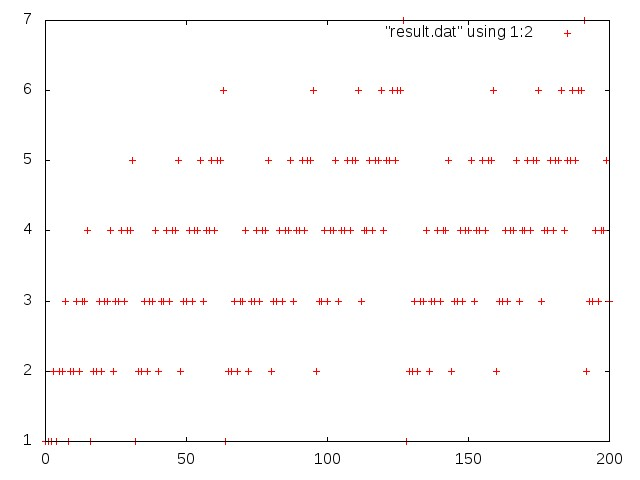
\includegraphics{plot}}
\end{center}

An analysis of the code itself explains the empirical results when we
observe that there is no direct correlation between $T(n)$ and $n$ except
for the fact that as $n$ grows larger, $T(n)$ seems to fluctuate
more drastically. An examination of the algorithm indicates that the number
of basic operations, $T(n)$, is proportional to the number of set bits in
the binary representation of $n$. This supports the earlier observation, 
since the larger $n$ is, the larger the maximum possible value of $T(n)$ 
is since the maximum number of set bits in $n$ is higher. Assume that n is 
strictly positive, $T(n)$ is bounded from below by $1$ and from above by 
the total number of bits in the binary representation of $n$, 
$\left \lceil {log_2n} \right \rceil$ where the ceiling function 
$\left \lceil {x} \right \rceil$ denotes the smallest integer greater than 
or equal to x. The lower bound occurs when $n$ is a power of 2 while the 
upper bound occurs when $n$ is 1 less than a power of 2. This is empirically 
corroborated by the above graph, in which $T(n)$ lies neatly between the 
logarithmic curve $f(n) = log_2n$ and the horizontal line $y = 1$.

Therefore, we conclude that this algorithm is described by

\[
T(n) \in \Omega( 1 ) \land T(n) \in O(log_2n)
\]

\end{document}
